\documentclass[]{article}
\usepackage{lmodern}
\usepackage{amssymb,amsmath}
\usepackage{ifxetex,ifluatex}
\usepackage{fixltx2e} % provides \textsubscript
\ifnum 0\ifxetex 1\fi\ifluatex 1\fi=0 % if pdftex
  \usepackage[T1]{fontenc}
  \usepackage[utf8]{inputenc}
\else % if luatex or xelatex
  \ifxetex
    \usepackage{mathspec}
  \else
    \usepackage{fontspec}
  \fi
  \defaultfontfeatures{Ligatures=TeX,Scale=MatchLowercase}
\fi
% use upquote if available, for straight quotes in verbatim environments
\IfFileExists{upquote.sty}{\usepackage{upquote}}{}
% use microtype if available
\IfFileExists{microtype.sty}{%
\usepackage{microtype}
\UseMicrotypeSet[protrusion]{basicmath} % disable protrusion for tt fonts
}{}
\usepackage[margin=1in]{geometry}
\usepackage{hyperref}
\hypersetup{unicode=true,
            pdftitle={DATA 606 - Lab2},
            pdfauthor={Joshua Sturm},
            pdfborder={0 0 0},
            breaklinks=true}
\urlstyle{same}  % don't use monospace font for urls
\usepackage{color}
\usepackage{fancyvrb}
\newcommand{\VerbBar}{|}
\newcommand{\VERB}{\Verb[commandchars=\\\{\}]}
\DefineVerbatimEnvironment{Highlighting}{Verbatim}{commandchars=\\\{\}}
% Add ',fontsize=\small' for more characters per line
\usepackage{framed}
\definecolor{shadecolor}{RGB}{248,248,248}
\newenvironment{Shaded}{\begin{snugshade}}{\end{snugshade}}
\newcommand{\KeywordTok}[1]{\textcolor[rgb]{0.13,0.29,0.53}{\textbf{{#1}}}}
\newcommand{\DataTypeTok}[1]{\textcolor[rgb]{0.13,0.29,0.53}{{#1}}}
\newcommand{\DecValTok}[1]{\textcolor[rgb]{0.00,0.00,0.81}{{#1}}}
\newcommand{\BaseNTok}[1]{\textcolor[rgb]{0.00,0.00,0.81}{{#1}}}
\newcommand{\FloatTok}[1]{\textcolor[rgb]{0.00,0.00,0.81}{{#1}}}
\newcommand{\ConstantTok}[1]{\textcolor[rgb]{0.00,0.00,0.00}{{#1}}}
\newcommand{\CharTok}[1]{\textcolor[rgb]{0.31,0.60,0.02}{{#1}}}
\newcommand{\SpecialCharTok}[1]{\textcolor[rgb]{0.00,0.00,0.00}{{#1}}}
\newcommand{\StringTok}[1]{\textcolor[rgb]{0.31,0.60,0.02}{{#1}}}
\newcommand{\VerbatimStringTok}[1]{\textcolor[rgb]{0.31,0.60,0.02}{{#1}}}
\newcommand{\SpecialStringTok}[1]{\textcolor[rgb]{0.31,0.60,0.02}{{#1}}}
\newcommand{\ImportTok}[1]{{#1}}
\newcommand{\CommentTok}[1]{\textcolor[rgb]{0.56,0.35,0.01}{\textit{{#1}}}}
\newcommand{\DocumentationTok}[1]{\textcolor[rgb]{0.56,0.35,0.01}{\textbf{\textit{{#1}}}}}
\newcommand{\AnnotationTok}[1]{\textcolor[rgb]{0.56,0.35,0.01}{\textbf{\textit{{#1}}}}}
\newcommand{\CommentVarTok}[1]{\textcolor[rgb]{0.56,0.35,0.01}{\textbf{\textit{{#1}}}}}
\newcommand{\OtherTok}[1]{\textcolor[rgb]{0.56,0.35,0.01}{{#1}}}
\newcommand{\FunctionTok}[1]{\textcolor[rgb]{0.00,0.00,0.00}{{#1}}}
\newcommand{\VariableTok}[1]{\textcolor[rgb]{0.00,0.00,0.00}{{#1}}}
\newcommand{\ControlFlowTok}[1]{\textcolor[rgb]{0.13,0.29,0.53}{\textbf{{#1}}}}
\newcommand{\OperatorTok}[1]{\textcolor[rgb]{0.81,0.36,0.00}{\textbf{{#1}}}}
\newcommand{\BuiltInTok}[1]{{#1}}
\newcommand{\ExtensionTok}[1]{{#1}}
\newcommand{\PreprocessorTok}[1]{\textcolor[rgb]{0.56,0.35,0.01}{\textit{{#1}}}}
\newcommand{\AttributeTok}[1]{\textcolor[rgb]{0.77,0.63,0.00}{{#1}}}
\newcommand{\RegionMarkerTok}[1]{{#1}}
\newcommand{\InformationTok}[1]{\textcolor[rgb]{0.56,0.35,0.01}{\textbf{\textit{{#1}}}}}
\newcommand{\WarningTok}[1]{\textcolor[rgb]{0.56,0.35,0.01}{\textbf{\textit{{#1}}}}}
\newcommand{\AlertTok}[1]{\textcolor[rgb]{0.94,0.16,0.16}{{#1}}}
\newcommand{\ErrorTok}[1]{\textcolor[rgb]{0.64,0.00,0.00}{\textbf{{#1}}}}
\newcommand{\NormalTok}[1]{{#1}}
\usepackage{graphicx,grffile}
\makeatletter
\def\maxwidth{\ifdim\Gin@nat@width>\linewidth\linewidth\else\Gin@nat@width\fi}
\def\maxheight{\ifdim\Gin@nat@height>\textheight\textheight\else\Gin@nat@height\fi}
\makeatother
% Scale images if necessary, so that they will not overflow the page
% margins by default, and it is still possible to overwrite the defaults
% using explicit options in \includegraphics[width, height, ...]{}
\setkeys{Gin}{width=\maxwidth,height=\maxheight,keepaspectratio}
\IfFileExists{parskip.sty}{%
\usepackage{parskip}
}{% else
\setlength{\parindent}{0pt}
\setlength{\parskip}{6pt plus 2pt minus 1pt}
}
\setlength{\emergencystretch}{3em}  % prevent overfull lines
\providecommand{\tightlist}{%
  \setlength{\itemsep}{0pt}\setlength{\parskip}{0pt}}
\setcounter{secnumdepth}{0}
% Redefines (sub)paragraphs to behave more like sections
\ifx\paragraph\undefined\else
\let\oldparagraph\paragraph
\renewcommand{\paragraph}[1]{\oldparagraph{#1}\mbox{}}
\fi
\ifx\subparagraph\undefined\else
\let\oldsubparagraph\subparagraph
\renewcommand{\subparagraph}[1]{\oldsubparagraph{#1}\mbox{}}
\fi

%%% Use protect on footnotes to avoid problems with footnotes in titles
\let\rmarkdownfootnote\footnote%
\def\footnote{\protect\rmarkdownfootnote}

%%% Change title format to be more compact
\usepackage{titling}

% Create subtitle command for use in maketitle
\newcommand{\subtitle}[1]{
  \posttitle{
    \begin{center}\large#1\end{center}
    }
}

\setlength{\droptitle}{-2em}
  \title{DATA 606 - Lab2}
  \pretitle{\vspace{\droptitle}\centering\huge}
  \posttitle{\par}
  \author{Joshua Sturm}
  \preauthor{\centering\large\emph}
  \postauthor{\par}
  \predate{\centering\large\emph}
  \postdate{\par}
  \date{09/07/2017}


\begin{document}
\maketitle

\subsection{Getting Started}\label{getting-started}

Our investigation will focus on the performance of one player: Kobe
Bryant of the Los Angeles Lakers. His performance against the Orlando
Magic in the 2009 NBA finals earned him the title \emph{Most Valuable
Player} and many spectators commented on how he appeared to show a hot
hand. Let's load some data from those games and look at the first
several rows.

\begin{Shaded}
\begin{Highlighting}[]
\KeywordTok{load}\NormalTok{(}\StringTok{"more/kobe.RData"}\NormalTok{)}
\KeywordTok{head}\NormalTok{(kobe)}
\end{Highlighting}
\end{Shaded}

\begin{verbatim}
##    vs game quarter time
## 1 ORL    1       1 9:47
## 2 ORL    1       1 9:07
## 3 ORL    1       1 8:11
## 4 ORL    1       1 7:41
## 5 ORL    1       1 7:03
## 6 ORL    1       1 6:01
##                                               description basket
## 1                 Kobe Bryant makes 4-foot two point shot      H
## 2                               Kobe Bryant misses jumper      M
## 3                        Kobe Bryant misses 7-foot jumper      M
## 4 Kobe Bryant makes 16-foot jumper (Derek Fisher assists)      H
## 5                         Kobe Bryant makes driving layup      H
## 6                               Kobe Bryant misses jumper      M
\end{verbatim}

In this data frame, every row records a shot taken by Kobe Bryant. If he
hit the shot (made a basket), a hit, \texttt{H}, is recorded in the
column named \texttt{basket}, otherwise a miss, \texttt{M}, is recorded.

Just looking at the string of hits and misses, it can be difficult to
gauge whether or not it seems like Kobe was shooting with a hot hand.
One way we can approach this is by considering the belief that hot hand
shooters tend to go on shooting streaks. For this lab, we define the
length of a shooting streak to be the \emph{number of consecutive
baskets made until a miss occurs}.

For example, in Game 1 Kobe had the following sequence of hits and
misses from his nine shot attempts in the first quarter:

\[ \textrm{H M | M | H H M | M | M | M} \]

To verify this use the following command:

\begin{Shaded}
\begin{Highlighting}[]
\NormalTok{kobe$basket[}\DecValTok{1}\NormalTok{:}\DecValTok{9}\NormalTok{]}
\end{Highlighting}
\end{Shaded}

\begin{verbatim}
## [1] "H" "M" "M" "H" "H" "M" "M" "M" "M"
\end{verbatim}

Within the nine shot attempts, there are six streaks, which are
separated by a ``\textbar{}'' above. Their lengths are one, zero, two,
zero, zero, zero (in order of occurrence).

\begin{enumerate}
\def\labelenumi{\arabic{enumi}.}
\tightlist
\item
  What does a streak length of 1 mean, i.e.~how many hits and misses are
  in a streak of 1? What about a streak length of 0?
\end{enumerate}

\begin{verbatim}
A streak of 1 would simply be only one consecutive hit. A streak of 0 would be a miss.
\end{verbatim}

The custom function \texttt{calc\_streak}, which was loaded in with the
data, may be used to calculate the lengths of all shooting streaks and
then look at the distribution.

\begin{Shaded}
\begin{Highlighting}[]
\NormalTok{kobe_streak <-}\StringTok{ }\KeywordTok{calc_streak}\NormalTok{(kobe$basket)}
\KeywordTok{barplot}\NormalTok{(}\KeywordTok{table}\NormalTok{(kobe_streak))}
\end{Highlighting}
\end{Shaded}

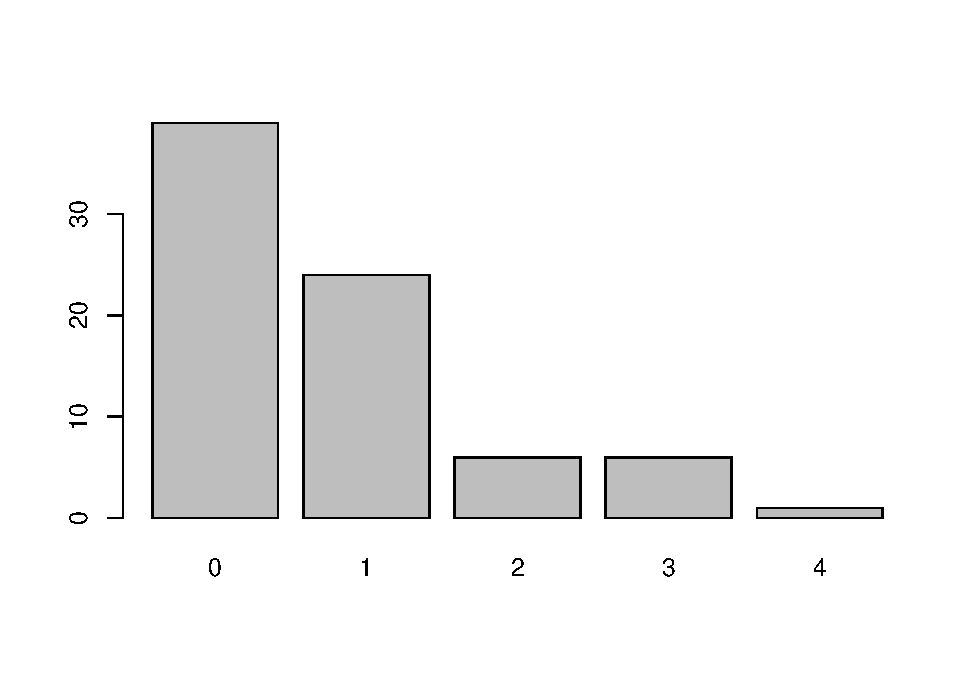
\includegraphics{Lab2_files/figure-latex/calc-streak-kobe-1.pdf}

Note that instead of making a histogram, we chose to make a bar plot
from a table of the streak data. A bar plot is preferable here since our
variable is discrete -- counts -- instead of continuous.

\begin{enumerate}
\def\labelenumi{\arabic{enumi}.}
\setcounter{enumi}{1}
\tightlist
\item
  Describe the distribution of Kobe's streak lengths from the 2009 NBA
  finals. What was his typical streak length? How long was his longest
  streak of baskets?
\end{enumerate}

\begin{verbatim}
It's right skewed, in that the majority were misses, with very few actual hit streaks. The typical streak was of length 1. His longest streak was 4 consecutive hits.
\end{verbatim}

\subsection{Compared to What?}\label{compared-to-what}

We've shown that Kobe had some long shooting streaks, but are they long
enough to support the belief that he had hot hands? What can we compare
them to?

To answer these questions, let's return to the idea of
\emph{independence}. Two processes are independent if the outcome of one
process doesn't effect the outcome of the second. If each shot that a
player takes is an independent process, having made or missed your first
shot will not affect the probability that you will make or miss your
second shot.

A shooter with a hot hand will have shots that are \emph{not}
independent of one another. Specifically, if the shooter makes his first
shot, the hot hand model says he will have a \emph{higher} probability
of making his second shot.

Let's suppose for a moment that the hot hand model is valid for Kobe.
During his career, the percentage of time Kobe makes a basket (i.e.~his
shooting percentage) is about 45\%, or in probability notation,

\[ P(\textrm{shot 1 = H}) = 0.45 \]

If he makes the first shot and has a hot hand (\emph{not} independent
shots), then the probability that he makes his second shot would go up
to, let's say, 60\%,

\[ P(\textrm{shot 2 = H} \, | \, \textrm{shot 1 = H}) = 0.60 \]

As a result of these increased probabilites, you'd expect Kobe to have
longer streaks. Compare this to the skeptical perspective where Kobe
does \emph{not} have a hot hand, where each shot is independent of the
next. If he hit his first shot, the probability that he makes the second
is still 0.45.

\[ P(\textrm{shot 2 = H} \, | \, \textrm{shot 1 = H}) = 0.45 \]

In other words, making the first shot did nothing to affect the
probability that he'd make his second shot. If Kobe's shots are
independent, then he'd have the same probability of hitting every shot
regardless of his past shots: 45\%.

Now that we've phrased the situation in terms of independent shots,
let's return to the question: how do we tell if Kobe's shooting streaks
are long enough to indicate that he has hot hands? We can compare his
streak lengths to someone without hot hands: an independent shooter.

\subsection{Simulations in R}\label{simulations-in-r}

While we don't have any data from a shooter we know to have independent
shots, that sort of data is very easy to simulate in R. In a simulation,
you set the ground rules of a random process and then the computer uses
random numbers to generate an outcome that adheres to those rules. As a
simple example, you can simulate flipping a fair coin with the
following.

\begin{Shaded}
\begin{Highlighting}[]
\NormalTok{outcomes <-}\StringTok{ }\KeywordTok{c}\NormalTok{(}\StringTok{"heads"}\NormalTok{, }\StringTok{"tails"}\NormalTok{)}
\KeywordTok{sample}\NormalTok{(outcomes, }\DataTypeTok{size =} \DecValTok{1}\NormalTok{, }\DataTypeTok{replace =} \OtherTok{TRUE}\NormalTok{)}
\end{Highlighting}
\end{Shaded}

\begin{verbatim}
## [1] "heads"
\end{verbatim}

The vector \texttt{outcomes} can be thought of as a hat with two slips
of paper in it: one slip says \texttt{heads} and the other says
\texttt{tails}. The function \texttt{sample} draws one slip from the hat
and tells us if it was a head or a tail.

Run the second command listed above several times. Just like when
flipping a coin, sometimes you'll get a heads, sometimes you'll get a
tails, but in the long run, you'd expect to get roughly equal numbers of
each.

If you wanted to simulate flipping a fair coin 100 times, you could
either run the function 100 times or, more simply, adjust the
\texttt{size} argument, which governs how many samples to draw (the
\texttt{replace\ =\ TRUE} argument indicates we put the slip of paper
back in the hat before drawing again). Save the resulting vector of
heads and tails in a new object called \texttt{sim\_fair\_coin}.

\begin{Shaded}
\begin{Highlighting}[]
\NormalTok{sim_fair_coin <-}\StringTok{ }\KeywordTok{sample}\NormalTok{(outcomes, }\DataTypeTok{size =} \DecValTok{100}\NormalTok{, }\DataTypeTok{replace =} \OtherTok{TRUE}\NormalTok{)}
\end{Highlighting}
\end{Shaded}

To view the results of this simulation, type the name of the object and
then use \texttt{table} to count up the number of heads and tails.

\begin{Shaded}
\begin{Highlighting}[]
\NormalTok{sim_fair_coin}
\end{Highlighting}
\end{Shaded}

\begin{verbatim}
##   [1] "tails" "tails" "tails" "heads" "tails" "heads" "heads" "tails"
##   [9] "tails" "heads" "heads" "heads" "tails" "heads" "heads" "tails"
##  [17] "heads" "heads" "tails" "heads" "tails" "tails" "heads" "tails"
##  [25] "tails" "heads" "heads" "heads" "tails" "heads" "tails" "heads"
##  [33] "heads" "tails" "tails" "heads" "heads" "heads" "tails" "heads"
##  [41] "tails" "tails" "heads" "heads" "tails" "tails" "tails" "heads"
##  [49] "heads" "tails" "tails" "heads" "heads" "heads" "heads" "tails"
##  [57] "tails" "tails" "heads" "tails" "heads" "tails" "tails" "tails"
##  [65] "heads" "heads" "heads" "heads" "tails" "heads" "tails" "heads"
##  [73] "tails" "heads" "tails" "tails" "heads" "tails" "tails" "tails"
##  [81] "tails" "tails" "tails" "tails" "heads" "heads" "tails" "tails"
##  [89] "tails" "tails" "tails" "tails" "tails" "tails" "tails" "tails"
##  [97] "heads" "heads" "heads" "tails"
\end{verbatim}

\begin{Shaded}
\begin{Highlighting}[]
\KeywordTok{table}\NormalTok{(sim_fair_coin)}
\end{Highlighting}
\end{Shaded}

\begin{verbatim}
## sim_fair_coin
## heads tails 
##    45    55
\end{verbatim}

Since there are only two elements in \texttt{outcomes}, the probability
that we ``flip'' a coin and it lands heads is 0.5. Say we're trying to
simulate an unfair coin that we know only lands heads 20\% of the time.
We can adjust for this by adding an argument called \texttt{prob}, which
provides a vector of two probability weights.

\begin{Shaded}
\begin{Highlighting}[]
\NormalTok{sim_unfair_coin <-}\StringTok{ }\KeywordTok{sample}\NormalTok{(outcomes, }\DataTypeTok{size =} \DecValTok{100}\NormalTok{, }\DataTypeTok{replace =} \OtherTok{TRUE}\NormalTok{, }\DataTypeTok{prob =} \KeywordTok{c}\NormalTok{(}\FloatTok{0.2}\NormalTok{, }\FloatTok{0.8}\NormalTok{))}
\end{Highlighting}
\end{Shaded}

\texttt{prob=c(0.2,\ 0.8)} indicates that for the two elements in the
\texttt{outcomes} vector, we want to select the first one,
\texttt{heads}, with probability 0.2 and the second one, \texttt{tails}
with probability 0.8. Another way of thinking about this is to think of
the outcome space as a bag of 10 chips, where 2 chips are labeled
``head'' and 8 chips ``tail''. Therefore at each draw, the probability
of drawing a chip that says ``head''" is 20\%, and ``tail'' is 80\%.

\begin{enumerate}
\def\labelenumi{\arabic{enumi}.}
\setcounter{enumi}{2}
\tightlist
\item
  In your simulation of flipping the unfair coin 100 times, how many
  flips came up heads?
\end{enumerate}

\begin{Shaded}
\begin{Highlighting}[]
\NormalTok{sim_unfair_coin <-}\StringTok{ }\KeywordTok{sample}\NormalTok{(outcomes, }\DataTypeTok{size =} \DecValTok{100}\NormalTok{, }\DataTypeTok{replace =} \OtherTok{TRUE}\NormalTok{, }\DataTypeTok{prob =} \KeywordTok{c}\NormalTok{(}\FloatTok{0.2}\NormalTok{, }\FloatTok{0.8}\NormalTok{))}
\KeywordTok{table}\NormalTok{(sim_unfair_coin)}
\end{Highlighting}
\end{Shaded}

\begin{verbatim}
## sim_unfair_coin
## heads tails 
##    19    81
\end{verbatim}

\subsection{Simulating the Independent
Shooter}\label{simulating-the-independent-shooter}

Simulating a basketball player who has independent shots uses the same
mechanism that we use to simulate a coin flip. To simulate a single shot
from an independent shooter with a shooting percentage of 50\% we type,

\begin{Shaded}
\begin{Highlighting}[]
\NormalTok{outcomes <-}\StringTok{ }\KeywordTok{c}\NormalTok{(}\StringTok{"H"}\NormalTok{, }\StringTok{"M"}\NormalTok{)}
\NormalTok{sim_basket <-}\StringTok{ }\KeywordTok{sample}\NormalTok{(outcomes, }\DataTypeTok{size =} \DecValTok{1}\NormalTok{, }\DataTypeTok{replace =} \OtherTok{TRUE}\NormalTok{)}
\end{Highlighting}
\end{Shaded}

To make a valid comparison between Kobe and our simulated independent
shooter, we need to align both their shooting percentage and the number
of attempted shots.

\begin{enumerate}
\def\labelenumi{\arabic{enumi}.}
\setcounter{enumi}{3}
\tightlist
\item
  What change needs to be made to the \texttt{sample} function so that
  it reflects a shooting percentage of 45\%? Make this adjustment, then
  run a simulation to sample 133 shots. Assign the output of this
  simulation to a new object called \texttt{sim\_basket}.
\end{enumerate}

\begin{Shaded}
\begin{Highlighting}[]
\KeywordTok{set.seed}\NormalTok{(}\DecValTok{472}\NormalTok{)}
\NormalTok{sim_basket <-}\StringTok{ }\KeywordTok{sample}\NormalTok{(outcomes, }\DataTypeTok{size =} \DecValTok{133}\NormalTok{, }\DataTypeTok{replace =} \OtherTok{TRUE}\NormalTok{, }\DataTypeTok{prob=}\KeywordTok{c}\NormalTok{(}\FloatTok{0.45}\NormalTok{, }\FloatTok{0.55}\NormalTok{))}
\KeywordTok{table}\NormalTok{(sim_basket)}
\end{Highlighting}
\end{Shaded}

\begin{verbatim}
## sim_basket
##  H  M 
## 73 60
\end{verbatim}

\begin{verbatim}
We can customize the probability for each variable with the prob() function.
I used the function 'set.seed' to make the data reproducible.
\end{verbatim}

With the results of the simulation saved as \texttt{sim\_basket}, we
have the data necessary to compare Kobe to our independent shooter. We
can look at Kobe's data alongside our simulated data.

\begin{Shaded}
\begin{Highlighting}[]
\KeywordTok{table}\NormalTok{(kobe$basket)}
\end{Highlighting}
\end{Shaded}

\begin{verbatim}
## 
##  H  M 
## 58 75
\end{verbatim}

Both data sets represent the results of 133 shot attempts, each with the
same shooting percentage of 45\%. We know that our simulated data is
from a shooter that has independent shots. That is, we know the
simulated shooter does not have a hot hand.

\begin{center}\rule{0.5\linewidth}{\linethickness}\end{center}

\subsection{On your own}\label{on-your-own}

\subsubsection{Comparing Kobe Bryant to the Independent
Shooter}\label{comparing-kobe-bryant-to-the-independent-shooter}

Using \texttt{calc\_streak}, compute the streak lengths of
\texttt{sim\_basket}.

\begin{Shaded}
\begin{Highlighting}[]
\NormalTok{sim_streak <-}\StringTok{ }\KeywordTok{calc_streak}\NormalTok{(sim_basket)}
\end{Highlighting}
\end{Shaded}

\begin{verbatim}
I calculated the streak for our simulated player, and assigned it to a new variable 'sim_streak'
\end{verbatim}

\begin{enumerate}
\def\labelenumi{\arabic{enumi}.}
\tightlist
\item
  Describe the distribution of streak lengths. What is the typical
  streak length for this simulated independent shooter with a 45\%
  shooting percentage? How long is the player's longest streak of
  baskets in 133 shots?
\end{enumerate}

\begin{Shaded}
\begin{Highlighting}[]
\KeywordTok{barplot}\NormalTok{(}\KeywordTok{table}\NormalTok{(sim_streak))}
\end{Highlighting}
\end{Shaded}

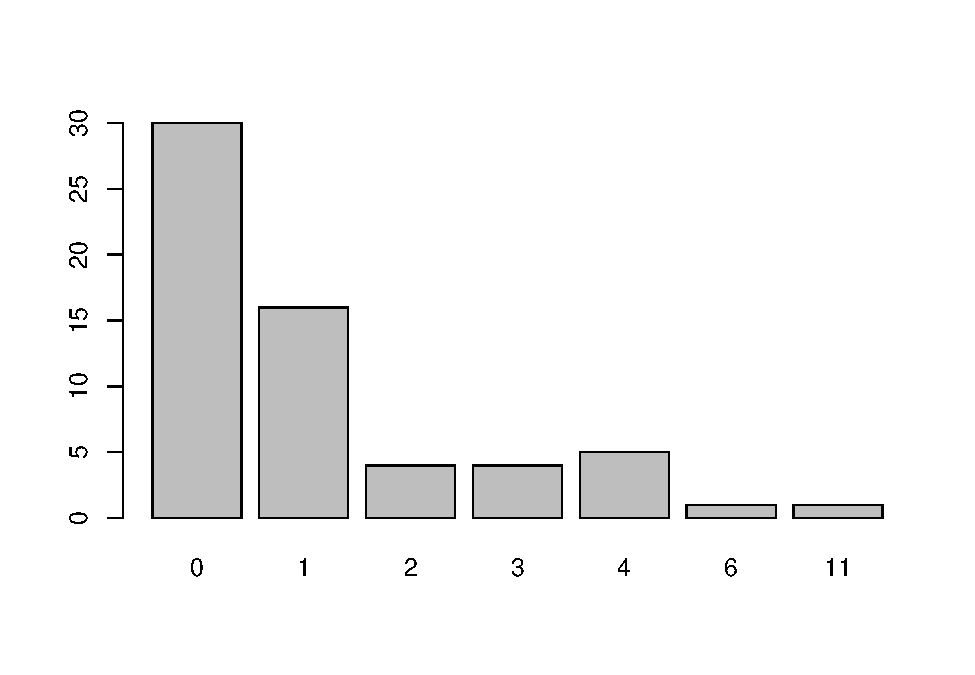
\includegraphics{Lab2_files/figure-latex/unnamed-chunk-4-1.pdf}

\begin{verbatim}
The distribution is unimodal and right skewed. The majority of shots were misses (i.e. streak of 0). The longest streak was 11 hits in a row.
\end{verbatim}

\begin{enumerate}
\def\labelenumi{\arabic{enumi}.}
\setcounter{enumi}{1}
\tightlist
\item
  If you were to run the simulation of the independent shooter a second
  time, how would you expect its streak distribution to compare to the
  distribution from the question above? Exactly the same? Somewhat
  similar? Totally different? Explain your reasoning.
\end{enumerate}

\begin{verbatim}
Assuming we didn't use 'set.seed' in both runs, we would get slightly different results, but they'd be very close. We've established that the shots are independent of each other, so the distribution would be similar.
\end{verbatim}

\begin{enumerate}
\def\labelenumi{\arabic{enumi}.}
\setcounter{enumi}{2}
\tightlist
\item
  How does Kobe Bryant's distribution of streak lengths compare to the
  distribution of streak lengths for the simulated shooter? Using this
  comparison, do you have evidence that the hot hand model fits Kobe's
  shooting patterns? Explain.
\end{enumerate}

\begin{Shaded}
\begin{Highlighting}[]
\KeywordTok{par}\NormalTok{(}\DataTypeTok{mfrow=}\KeywordTok{c}\NormalTok{(}\DecValTok{1}\NormalTok{,}\DecValTok{2}\NormalTok{))}
\KeywordTok{barplot}\NormalTok{(}\KeywordTok{table}\NormalTok{(kobe_streak))}
\KeywordTok{barplot}\NormalTok{(}\KeywordTok{table}\NormalTok{(sim_streak))}
\end{Highlighting}
\end{Shaded}

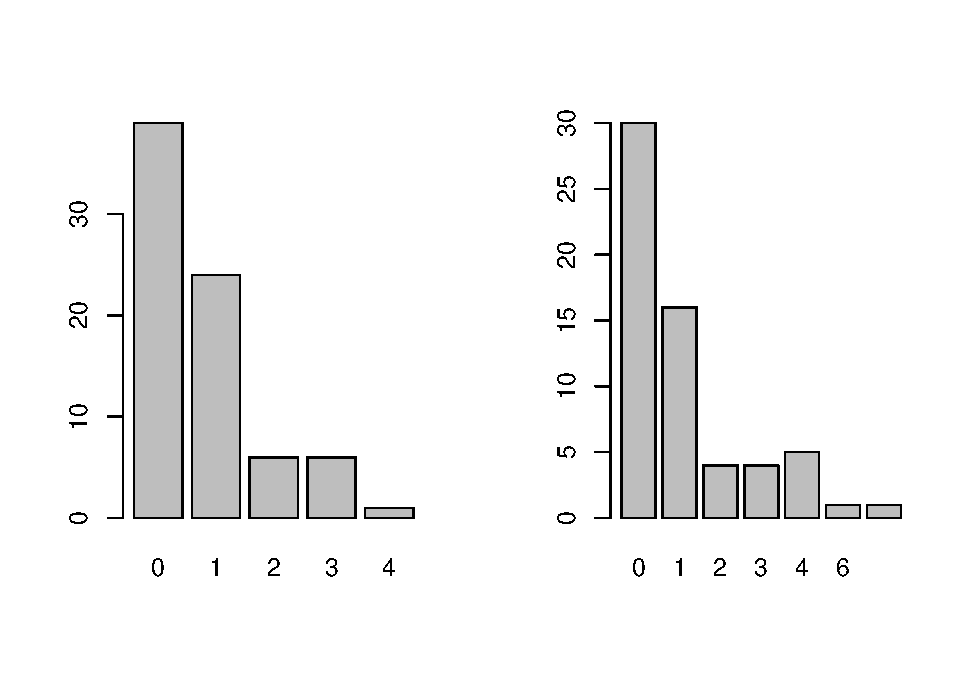
\includegraphics{Lab2_files/figure-latex/unnamed-chunk-5-1.pdf}

\begin{verbatim}
While the independent shooter had some longer streaks, overall, the distributions of his and kobe's shot patterns are similar: both are right skewed and unimodal. We can conclude from this that the hot hand theory does not hold, and the shots are indeed independent of each other.
\end{verbatim}


\end{document}
